\chapter{Sets}
\label{chapter:sets}
\marginurl{%
  Sets:\\\noindent
  Introduction to Mathematical Reasoning \#6
}{youtu.be/bshBV2H4Sqo}
\section{The Intuitive Definition of a Set}
A set is one of the two most important concepts in mathematics. Many mathematical
statements involve ``an integer $n$'' or ``a real number $a$''. Set theory
notation provides a simple way to express that $a$ is a real number. However,
this language is much more expressible and it is impossible to imagine modern
mathematics without this notation.

As in the previous chapter it is difficult to define a set formally so we give
a less formal definition which should be enough to use the notation.
A \emph{set} is a well-defined collection of objects. Important examples of
sets are:
\begin{enumerate}
  \item $\R$ a set of reals,
    \nomenclature[S]{$\R$}{denotes the set of all real numbers}
  \item $\Z$ the set of integers\footnote{``Z'' stands for the German word
    Zahlen (``numbers'').},
    \nomenclature[S]{$\Z$}{denotes the set of all integers}
  \item $\N$ the set of natural numbers\footnote{Note that in the literature
      there are two different traditions: in one $0$ is a natural number, in
      another it is not; in this book we are going to assume that $0$ is not a
      natural number.
    },
    \nomenclature[S]{$\N$}{denotes the set of all integers greater
    than $0$}
  \item $\Q$ a set of rational numbers,
    \nomenclature[S]{$\Q$}{denotes the set of all rational numbers}
  \item $\mathbb{C}$ a set of complex numbers.
    \nomenclature[S]{$\C$}{denotes the set of all complex numbers}
\end{enumerate}
Usually, sets are denoted by a single letter.

Objects in a set are called \emph{elements} of the set and we denote the
statement ``x is in the set $E$'' by the formula $x \in E$ and the negation of
this statement by $x \not\in E$. For example, we proved that
$\sqrt{2} \not\in \Q$\footnote{%
  The symbol $\in$ was first used by Giuseppe Peano 1889 in his work
  ``Arithmetices principia, nova methodo exposita''. Here he wrote on page X:
  ``The symbol $\in$ means is. So $a \in b$ is read as a \emph{is} a b;
  \dots''
  The symbol itself is a stylized lowercase Greek letter epsilon
  (``$\epsilon$''), the first letter of the word  \textgreek{esti}, which means
  ``is''.
}.

\begin{exercise}
  \label{exercise:inclusion}

  Which of the following sets are included in which? Recall that a number is
  prime iff it is an integer greater than $1$ and divisible only by $1$ and
  itself.
  \begin{enumerate}
    \item The set of all positive integers less than $10$.
    \item The set of all prime numbers less than $11$.
    \item The set of all odd numbers greater than $1$ and less than $6$.
    \item The set of all positive integers less than $10$.
    \item The set whose only elements are $1$ and $2$.
    \item The set whose only element is $1$.
    \item The set of all prime numbers less than $11$.
  \end{enumerate}
\end{exercise}

\section{Basic Relations Between Sets}
Many problems in mathematics are problems of determining whether two descriptions
of sets are describing the same set or not. For example, when we learn how to
solve quadratic equations of the form $ax^2 + bx + c = 0$ ($a, b, c \in \R$) we
learn how to list the elements of the set $\set[ax^2 + bx + c = 0]{x \in \R}$.

We say that two sets $A$ and $B$ are equal if they contain the
same elements (we denote it by $A = B$). If all the elements of $A$ belong to
$B$ we say that $A$ is a subset of $B$ and denote it by
$A \subseteq B$\footnote{%
  In the literature there are three symbols for ``subset'': $\subseteq$,
  $\subsetneq$, and $\subset$. $A \subseteq B$ means that $A$ is a subset of
  $B$ and we allow $A = B$ and $A \subsetneq B$ means that $A$ is a subset of
  $B$ and we forbid $A = B$. However, there is a problem with the third symbol,
  some people use it as a synonym of $\subseteq$ and some use it as a synonym of
  $\subsetneq$. Due to this ambiguity we are going to avoid using it in this
  book.
}.

For example, $\Q \subseteq \R$ since any rational number is
also a real number. A special set is an empty set i.e. the set that does not
have elements, we denote it $\emptyset$.

\nomenclature[R]{$A \subseteq B$}{says that $A$ is a subset of $B$}

\nomenclature[S]{$\emptyset$}{denotes the set that does
  not have elements}

\subsection{Diagrams}
If we think of a set $A$ as represented by all the points within a circle or
any other closed figure, then it is easy to represent the notion of $A$ being a
subset of another set $B$ also represented by all the points within a circle.
We just put a circle labeled by $A$ inside of the circle labeled by $B$. We can
also diagram an equality by drawing a circle labeled by both $A$ and $B$. (see
fig.~\ref{figure:euler-diagram}). Such diagrams are called Euler diagrams and
it is clear that one may draw Euler diagrams for more than two sets.

\begin{figure}
    \centering
    \subfloat[$B \subseteq A$]{
      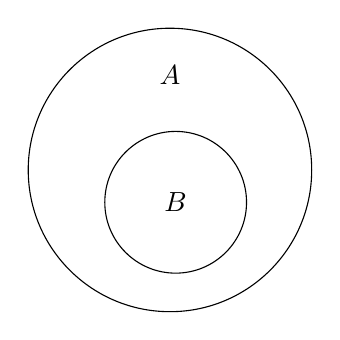
\begin{tikzpicture}[scale=0.6]
        \draw (20:2cm) circle (3cm) node [yshift=8ex] {$A$};
        \draw (0:2cm) circle (1.5cm) node {$B$};
      \end{tikzpicture}
    }
    \qquad\qquad
    \subfloat[$A = B$] {
      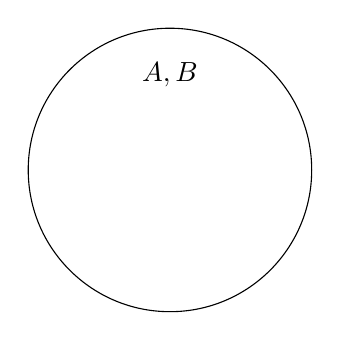
\begin{tikzpicture}[scale=0.6]
        \draw (20:2cm) circle (3cm) node [yshift=8ex] {$A, B$};
      \end{tikzpicture}
    }
    \caption{Euler diagrams for subset and equality relations}
    \label{figure:euler-diagram}
\end{figure}


\subsection{Descriptions of Sets}
In this section we describe how to define new sets, this notation is also
known as \emph{set-builder notation}.

\paragraph{Listing elements.} The simplest way to define a set is just to list
the elements. For example
\begin{enumerate}
  \item $\set{1, 2, \pi}$ is the set consisting of three elements 1, 2, and
    $\pi$, and
  \item $\set{1, 2, 3, \dots}$ is the set of all positive integers i.e. it is
    the set $\N$.
\end{enumerate}

\paragraph{Conditional definitions.}
We may also describe a set using some constraint e.g we may list all the even
numbers using the following formula $\set[n \text{ is even}]{n \in \Z}$
(we read it as ``the set of all integers $n$ such that $n$ is even'').

Using this we may also define the set of all integers from $1$ to $m$, we
denote it $[m]$; i.e. $[m] = \set[0 < n \le m]{n \in \N}$.
\nomenclature[S]{$[n]$}{denotes the set of all the integers from $1$ to n}


\paragraph{Constructive definitions.} Another way to construct a set of all
even numbers is to use the constructive definition of a set:
$\set[k \in \Z]{2k}$.

We may also describe a set of rational numbers using this description:
$\Q = \set[a \in \Z, b \in \N]{a / b}$ (note that we may also use a mix of
a conditional and constructive definitions,
$\Q = \set[a, b \in \Z, b \neq 0]{a / b}$).

\begin{exercise}
  Describe a set of perfect squares using constructive type of definition.
\end{exercise}

\subsection{Disjoint Sets}
Two sets are \emph{disjoint} iff they do not have common elements. We also
say that two sets are \emph{overlapping} iff they are not disjoint i.e. they
share at least one element.

More generally, $A_1$, \dots, $A_\ell$ are pairwise disjoint iff $A_i$ is
disjoint with $A_j$ for all $i \neq j \in [\ell]$

\begin{exercise}
  Of the sets in Exercise~\ref{exercise:inclusion}, which are disjoint from
  which?
\end{exercise}


\section{Operations over Sets.}
Another way to describe a set is to apply operation to other sets. Let $A$ and
$B$ be sets.
\begin{figure}
  \centering
  \subfloat[$A \cup B$]{
    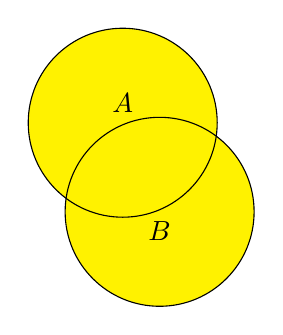
\begin{tikzpicture}[scale=0.8]
        \fill[yellow] (45:2cm) circle (1.5cm);
        \fill[yellow] (0:2cm) circle (1.5cm);

        \draw (45:2cm) circle (1.5cm) node [above] {$A$};
        \draw (0:2cm) circle (1.5cm) node [below] {$B$};
    \end{tikzpicture}
  }
  \qquad\qquad
  \subfloat[$A \cap B$]{
    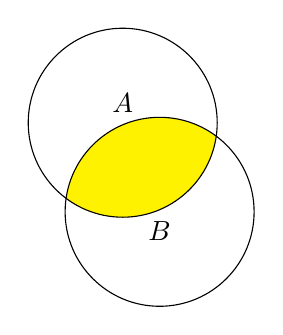
\begin{tikzpicture}[scale=0.8]
      \begin{scope}
          \clip (45:2cm) circle (1.5cm);
          \fill[yellow] (0:2cm) circle (1.5cm);
      \end{scope}
      \draw (45:2cm) circle (1.5cm) node [above] {$A$};
      \draw (0:2cm) circle (1.5cm) node [below] {$B$};
    \end{tikzpicture}
  }
  \vskip 0.25cm
  \subfloat[$A \setminus B$]{
    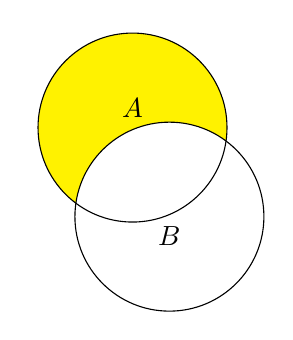
\begin{tikzpicture}[scale=0.8]
      \begin{scope}[even odd rule]
        \clip (0:2cm) circle (1.5cm) (-0.25,-0.25) rectangle (3,3);
        \fill[yellow] (45:2cm) circle (1.5cm);
      \end{scope}
      \draw (45:2cm) circle (1.5cm) node [above] {$A$};
      \draw (0:2cm) circle (1.5cm) node [below] {$B$};
    \end{tikzpicture}
  }
  \qquad\qquad
  \subfloat[$A \Delta B$]{
    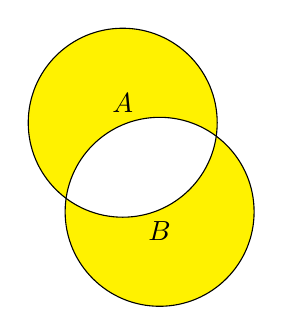
\begin{tikzpicture}[scale=0.8]
      \begin{scope}[even odd rule]
        \clip (0:2cm) circle (1.5cm) (45:2cm) circle (1.5cm);
        \fill[yellow] (45:2cm) circle (1.5cm);
        \fill[yellow] (0:2cm) circle (1.5cm);
      \end{scope}

      \draw (45:2cm) circle (1.5cm) node [above] {$A$};
      \draw (0:2cm) circle (1.5cm) node [below] {$B$};
    \end{tikzpicture}
  }
  \caption{Euler diagrams for set operations}
\end{figure}


The first example of the operations on sets is the \emph{union} operation.
The union of $A$ and $B$ is the set containing all the elements of $A$ and all
the elements of $B$ i.e.
$A \cup B = \set[x \in A \text{ or } x \in B]{x}$\footnote{%
  Note that this definition is not correct since in the conditional definitions
  we have to specify the set $x$ belongs to and we cannot do this here.
}.
\nomenclature[S]{$A \cup B$}{denotes the union of two sets $A$ and $B$}

Another example of such an operation is \emph{intersection}. The
intersection of $A$ and $B$ is the set of all the elements belonging to both
$A$ and $B$ i.e $A \cap B = \set[x \in A \text{ and } x \in B]{x}$\footnote{%
  You may notice that in the definition of the union we use disjunction and
  in the definition of intersection we use conjunction. Actually this is the
  reason the symbol of the conjunction is similar to the symbol of intersection
  and the symbol of the disjunction is similar to the symbol of union.
}.
\nomenclature[S]{$A \cap B$}{denotes the intersection of two sets $A$ and $B$}

The third operation we are going to discuss this lecture is
\emph{set difference}. If $A$ and $B$ are some sets, then
$A \setminus B = \set[x \in A \text{ and } x \not\in B]{x}$.
\nomenclature[S]{$A \setminus B$}{denotes the difference of two sets $A$ and $B$}

The last operation is \emph{symmetric difference}. If $A$ and $B$ are some
sets, then $A \Delta B = (A \setminus B) \cup (B \setminus A)$. Note that
alternatively $A \Delta B = (A \cup B) \setminus (A \cap B)$

\begin{exercise}
  Describe the set
  $\set[n \text{ is even}]{n \in \N} \cap \set[n \in \N]{3n}$.
\end{exercise}

\begin{theorem}
\label{theorem:set-equalities}
  Let $A$, $B$, and $C$ be some sets. Then we have the following identities.
  \begin{description}
    \item[(associativity)] $A \cup (B \cup C) = (A \cup B) \cup C$ and
      $A \cap (B \cap C) = (A \cap B) \cap C$.
    \item[(commutativity)] $A \cup B = B \cup A$ and $A \cap B = B \cap A$.
    \item[(distributivity)] $A \cup (B \cap C) = (A \cup B) \cap (A \cup C)$
      and $A \cap (B \cup C) = (A \cap B) \cup (A \cap C)$.
  \end{description}
\end{theorem}
\begin{proof}
  One may prove these properties using the Euler diagrams. Alternatively they
  can be proven by definitions. Let us prove only the first part of the
  distributivity, the rest is Exercise~\ref{exercise:set-equalities}.

  Our proof consists of two parts in the first part we prove that
  $A \cup (B \cap C) \subseteq (A \cup B) \cap (A \cup C)$.
  Suppose that $x \in A \cup (B \cap C)$. Then $x \in A$ or $x \in (B \cap C)$.
  \begin{itemize}
    \item If $x \in A$, then $x \in (A \cup B)$ and $x \in (A \cup C)$ i.e.
      $x \in ((A \cup B) \cap (A \cup C))$.
    \item If $x \in (B \cap C)$, then $x \in B$ and $x \in C$. Which implies
      that $x \in (A \cup B)$ and $x \in (A \cup C)$. As a result,
      $x \in ((A \cup B) \cap (A \cup C))$.
  \end{itemize}
\end{proof}

\begin{exercise}
\label{exercise:set-equalities}
  Prove the rest of the equalities in Theorem~\ref{theorem:set-equalities}.
\end{exercise}

Probably the most difficult concept connected to sets is
the concept of a power set. Let $A$ be some set, then the set of
all possible subsets of $A$ is denoted by $2^A$ (sometimes this set is denoted
by $\mathcal{P}(A)$) and called the power set of $A$. In other words $2^A =
\set[B \subseteq A]{B}$.

\nomenclature[S]{$2^A$}{denotes the set of all the subsets of the set $A$}

\begin{warning}
  Please do not forget about two extremal elements of the power set $2^A$: the
  empty set and $A$ itself.
\end{warning}

\noindent For example if $A = \set{1, 2, 3}$, then
\[
  2^A = \set{\emptyset, \set{1}, \set{2}, \set{3}, \set{1, 2},
  \set{1, 3}, \set{2, 3}, \set{1, 2, 3}}.
\]

\section{The Well-ordering Principle}
Using the set notation we may finally justify the proof of the statement
that $2^n > n$ for all positive integers $n$ from the video about mathematical
induction. In order to do this let us first formulate the following theorem.
\begin{theorem}
\label{theorem:well-ordering}
  Let $A \subseteq \Z$ be a non-empty set. We say that $b \in \Z$ is a lower
  bound for the set $A$ iff $b \le a$ for all $a \in A$. Additionally, we say
  that the set $A$ is bounded if there is a lower bound for $A$.

  Given this, if $A$ is bounded, then there is a lower bound $a \in A$ for the set $A$
  (we say that $a$ is the minimum of the set $A$).
\end{theorem}
Note that this theorem also states that any subset of natural numbers have a
minimum.

Recall that we wish to prove that $2^n > n$ for all positive $n$.
Assume that it is not true, in this case the set
$A = \set[2^n < n]{n \in \N}$ is non-empty. Denote by $n_0$ the minimum of the
set $A$, $n_0$ exists by Theorem~\ref{theorem:well-ordering}. We may consider
the following two cases.
\begin{itemize}
  \item If $n_0 = 1$, then it leads to a contradiction since $2 = 2^1 > 1$.
  \item Otherwise, note that $1 \le n_0 - 1 < n_0$, hence,
    $2^{n_0 - 1} > n_0 - 1$. So $2^{n_0} > 2n_0 - 2 \ge n_0$. Which is a
    contradiction with the definition of $n_0$.
\end{itemize}

Finally, we prove Theorem~\ref{theorem:well-ordering}.
\begin{proof}[Proof of Theorem~\ref{theorem:well-ordering}]
  Let $b$ be a lower bound for the set $A$. Assume that there is no minimum of
  the set $A$. Let $P(n)$ be the statement that
  $n \notin A$.

  First, we are going to prove that $P(n)$ is true for all
  $n \ge b$. The base case is true since if $b \in A$, then $b$ is the minimum
  of $A$ which contradicts to the assumption that there is no minimum of $A$.
  The induction step is also clear, by the induction hypothesis we know that
  $P(b)$, \dots, $P(k)$ are true, hence, $(k + 1) \in A$ implies that $k + 1$
  is the minimum of $A$.

  Now we prove that $A$ is empty. Assume the opposite i.e. assume that there is
  $x \in A$. Note that $x \ge b$ since $b$ is a lower bound of $A$. However,
  $P(x)$ is true which implies that $x \notin A$. Therefore the assumption was
  false and $A$ is empty, but this contradicts to the fact that $A$ is non-
  empty.
\end{proof}


\begin{chapterendexercises}
  \exercise Find the power sets of $\emptyset$, $\set{1}$, $\set{1, 2}$,
    $\set{1, 2, 3, 4}$. How many elements in each of this sets?
  \exercise[recommended] Prove that
    \begin{itemize}
      \item $A \subseteq B \iff A \cup B = B$,
      \item $A \subseteq B \iff A \cap B = A$.
    \end{itemize}
  \exercise Let $A$ be a subset of a set $U$ we call this set a universe.
    We say that the set $\overline{A} = U \setminus A$ is a complement of $A$
    in $U$. Show the following equalities
    \begin{itemize}
      \item $\overline{\overline{A}} = A$.
      \item $\overline{A \cup B} = \overline{A} \cap \overline{B}$.
      \item $\overline{A \cap B} = \overline{A} \cup \overline{B}$.
    \end{itemize}
  \exercise[recommended] Let us define an intersection of more than two sets as follows.
    Let $A_1$, \dots, $A_n$ be some sets. Then
    \begin{itemize}
      \item $\bigcap_{i = 1}^1 A_i = A_1$ and
      \item $\bigcap_{i = 1}^{k + 1} A_i = \left( \bigcap_{i = 1}^k A_i \right)
        \cap A_{k + 1}$.
    \end{itemize}
    \nomenclature[S]{$\bigcap_{i = 1}^k A_i$}{denotes $A_1 \cap \dots \cap
    A_k$}

    Show that $\bigcap_{i = 1}^n \set[i \le x \le n]{x \in \mathbb{N}} =
    \set{n}$ for all integers $n > 0$.
    \exercise Let us define a union of more than two sets as follows.
      Let $A_1$, \dots, $A_n$ be some sets. Then
      \begin{itemize}
        \item $\bigcup_{i = 1}^1 A_i = A_1$ and
        \item $\bigcup_{i = 1}^{k + 1} A_i =
          \left( \bigcup_{i = 1}^k A_i \right) \cup A_{k + 1}$.
      \end{itemize}
      \nomenclature[S]{$\bigcup_{i = 1}^k A_i$}{denotes $A_1 \cup \dots \cup
      A_k$}

      Show that $\bigcup_{i = 1}^n \range{i} = \range{n}$ for all integers $n > 0$.
  \exercise[recommended] Let $\Omega$ be some set and $A_1, \dots, A_n \subseteq \Omega$.
    Show that $\bigcup_{i = 1}^n A_i =
      \set[{\exists i \in \range{n}\ x \in A_i}]{x \in \Omega}$.
  \exercise Let $A_1$, \dots, $A_n$ be some sets.
    Show that $\bigcup_{i = 1}^n (A_i \cap B) =
    \left(\bigcup_{i = 1}^n A_i\right) \cap B$.
  \exercise Show that $A \Delta (B \Delta C) = (A \Delta B) \Delta C$.
  \exercise[recommended]
    Let $\mathbb{R}^{m \times n}$ be the set of all matrices $m \times n$ and
    $\mathbb{R}^n$ be the set of $n$ dimensional vectors.
    Show that for any matrix $A \in \mathbb{R}^{m \times n}$
    ($n > m$) there is a nonzero vector $x \in \mathbb{R}^n$ such that $Ax = 0$.
\end{chapterendexercises}
